\documentclass[12pt]{article}

\usepackage{discrete}

\def\thetitle{Introduction} % will be put in the center header on the first page only.
\def\lefthead{Math 228 Notes} % will be put in the left header
\def\righthead{Introduction} % will be put in the right header


\begin{document}

Welcome to Discrete Mathematics.  If this is your first time encountering the subject, you will probably find discrete mathematics quite different from other math subjects.  You might not even know what discrete math is!  Hopefully this short introduction will shed some light on what the subject is about and what you can expect as you move forward in your study of it.

\section{What is Discrete Mathematics?}

\begin{quotation}
\noindent \textbf{dis\textperiodcentered crete / dis\textquotesingle kr\={e}t}. \\ {\em Adjective}: Individually separate and distinct.  \\{\em Synonyms}: separate - detached - distinct - abstract.
\end{quotation}

Defining {\em discrete mathematics} is hard because defining {\em mathematics} is hard.  What is mathematics?  The study of numbers?  In part, yes.  But you also study functions and lines and triangles and parallelepipeds and vectors and \ldots.  Or perhaps you want to say that mathematics is a collection of tools that allow you to solve problems.  What sort of problems?  Okay, those that involve numbers, functions, lines, triangles,\ldots.  Whatever your conception of what mathematics is, try applying the concept of ``discrete'' to it, as defined above.  Some math fundamentally deals with \ldots {\em stuff} \ldots that is individually separate and distinct.  

In an algebra or calculus class, you might have found a particular set of numbers (maybe the set of number in the range of a function).  You would represent this set as an interval: $[0,\infty)$ is the range of $f(x) = x^2$ since the set of outputs of the function are all real numbers 0 and greater.  This set of numbers is \textbf{NOT} discrete.  The numbers in the set are not separated by much at all - in fact, take any two numbers in the set and there are infinitely many more between them which are also in the set.  Discrete math could still ask about the range of a function, but the set would not be an interval.  Consider the function which gives the number of children each person reading this has.  What is the range?  I'm guessing it is something like $\{0, 1, 2, 3\}$.  Maybe 4 is in there too.  But certainly there is nobody reading this that has 1.32419 children.  This set {\em is} discrete because the elements are separate.  Also notice that the inputs to the function are a discrete set - each input is an individual person - you would not consider fractional inputs (there is nothing $2/3$ between Bob and Carl we care about).  

One way to get a feel for the subject is to consider the types of problems you solve in discrete math.  Here are a few simple examples:

\begin{enumerate}
\item The most popular mathematician in the world is throwing a party for all of his friends.  As a way to kick things off, they decide that everyone should shake hands.  Assuming all 10 people at the party each shake hand with every other person (but not themselves, obviously) exactly once, how many handshakes take place?

\item At the warm-up event for Oscar's All Star Hot Dog Eating Contest, Al ate one hot dog.  Bob then showed him up by eating three hot dogs.  Not to be outdone, Carl ate five.  This continued with each contestant eating two more hot dogs than the previous contestant. How many hot dogs did Zeno (the 26th and final contestant) eat? How many hot dogs were eaten all together?

\item While walking through a fictional forest, you encounter three trolls.  Each is either a {\em knight}, who always tells the truth, or a {\em knave}, who always lies.  The trolls will not let you pass until you correctly identify each as either a knight or a knave.  Each troll makes a single statement:
  \begin{itemize}
   \item[] Troll 1: If I am a knave then there are exactly two knights here. 
   \item[] Troll 2: Troll 1 is lying.
   \item[] Troll 3: Either we are all knaves or at least one of us is a knight.
  \end{itemize}
Which troll is which? 

\item Back in the days of yore, five small towns decided they wanted to build roads directly connecting each pair of towns. While the towns had plenty of money to build roads as long and as winding as they wished, it was very important that the roads not intersect with each other (as stop signs had not yet been invented). Also, tunnels and bridges were not allowed. Is it possible for each of these town to build a road to each of the four other towns without creating any intersections? 
\end{enumerate}

One reason it is difficult to define discrete math is that it is a very broad description which encapsulates a large number of subjects.  In this course we will study four main topics: {\em combinatorics} (the theory of ways things {\em combine}, in particular, how to count these ways), {\em sequences}, {\em logic}, and {\em graph theory}.  However, there are other topics that belong under the discrete umbrella, including computer science, abstract algebra, number theory, game theory, probability, and geometry (some of these, particularly the last two, have both discrete and non-discrete variants).  

Ultimately the best way to learn what discrete math is about is to {\em do} it.  Let's get started! Before we can begin answering more complicated (and fun) problems, we must lay down some foundation.  We start by reviewing sets and functions in the framework of discrete mathematics.

\section{Sets}
\def\righthead{Sets}
\documentclass[12pt]{article}

\usepackage{../discrete}

\heading{Math 228}{}{Set Theory Notes}



\begin{document}

\section{Sets and Set Notation}

Here's a fun problem to think about.

\begin{problem}
An examination in three subjects, Algebra, Biology, and Chemistry, was taken
by 41 students. The following table shows how many students failed in each
single subject and in their various combinations.
\begin{center}
\begin{tabular}{|l|c|c|c|c|c|c|c|}
\hline
 Subject: & A & B & C & AB & AC & BC & ABC\\
\hline
Failed: & 12 & 5 & 8 & 2 & 6 & 3 & 1\\
\hline
\end{tabular}
\end{center}

How many students passed all three subjects?  Hint: the answer is not 4.
\end{problem}

What does this problem have to do with sets?  Well first maybe we should ask, what are sets?  This turns out to be a very hard question to answer precisely - in some sense sets are basic building blocks the same way that {\em points} are the basic building blocks in geometry.  For us however, it is safe to think of sets as simply a collection of objects.  For example, in the problem above, we might say that the 12 students to fail algebra form the {\em set} of students who failed algebra.  So the problem above really comes down to understanding how three sets interact.  

The set theory we will study is not complicated.\footnote{This is not to say that all set theory is easy - there are mathematicians who publish original research in set theory all the time.} However, there is a fair amount of new notation and terminology to learn.  Mastering these symbols and terms will allow us to use the language of set theory to help solve more complicated counting questions later on.

To help keep everything straight, the next page contains a sort of cheat sheet of the most important notation and terminology.  

\newpage
\begin{defbox}{Set Theory Notation}

\noindent  \begin{tabular}{l p{1.5in} p{3.5in}}
    Symbol: & Read: & Example: \\ \hline \\[1ex]
    $\{$, $\}$ & braces & $\{1,2,3\}$.  The braces enclose the elements of a set.  This is the set which contains the numbers 1, 2 and 3.\\[1ex]
    $\st$ & such that & $\{x \st x > 2\}$ is the set of all $x$ such that $x$ is greater than 2.\\[1ex]
    $\in$ & is an element of & $2 \in \{1,2,3\}$ asserts that 2 is one of the elements in the set $\{1,2,3\}$.  However, $4 \notin\{1,2,3\}$.\\[1ex]
    $\subseteq$ & is a subset of & $A \subseteq B$ asserts that every element of $A$ is also an element of $B$.\\[1ex]
    $\subset$ &is a proper subset of & $A \subset B$ asserts that every element of $A$ is also an element of $B$, but $A \ne B$.\\[1ex]
    $\cap$ & intersection & $A \cap B$ is the {\em set} of all elements which are elements of both $A$ and $B$.\\[1ex]
    $\cup$ & union & $A \cap B$ is the {\em set} of all elements which are elements of $A$ or $B$ or both.\\[1ex]
    $\setminus$ & set difference & $A \setminus B$ is the {\em set} of all elements of $A$ which are not elements of $B$.\\[1ex]
    $\bar A$ & compliment (of $A$) & $\bar A$ is the set of everything which is not an element of $A$.  The $A$ can be any set here.\\[1ex]
    $|A|$ & cardinality (of $A$)& $|\{4,5,6\}| = 3$ because there are 3 elements in the set.  Sometimes we say $|A|$ is the {\em size} of $A$.\\[1ex]
    
  \end{tabular}

\noindent{\bf Special sets}

\begin{tabular}{l p{5in}}
  $\emptyset$ & The {\em empty set} is the set which contains no elements.\\[1ex]
  $\U$ & The {\em universe set} is the set of all elements.\\[1ex]
$\N$ & The set of natural numbers. That is, $\N = \{0, 1, 2, 3\ldots\}$ \\[1ex]
$\Z$ & The set of integers.  $\Z = \{\ldots, -2, -1, 0, 1, 2, 3, \ldots\}$\\[1ex]
$\Q$ & The set of rational numbers.\\[1ex]
$\R$ & The set of real numbers.\\[1ex]
$\pow(A)$ & The {\em power set} of any set $A$ is the set of all subsets of $A$.
\end{tabular}


\end{defbox}

\newpage

\section{Basics}

For us, a set will simply be an unordered collection of objects.  For example, we could consider the set of all students enrolled at UNC this semester.  Or the set of natural numbers between 1 and 10 inclusive.  In the first case, each student here is a element (or member) of the set, while Barack Obama, among many others, is not an element of the set.  Also, the two example are of different sets.  Two sets are equal exactly if they contain the exact same elements.

Because we will want to consider many examples, we should have some notation to make talking about sets easier.  Consider,
\[ A = \{1, 2, 3\}.\]
This is read, ``$A$ is the set containing the elements 1, 2 and 3.''  We use curly braces ``$\{,~~ \}$'' to enclose elements of a set.  Some more notation:
\[ a \in \{a, b, c\}. \]
The symbol ``$\in$'' is read ``is in'' or ``is an element of.''  Thus the above means that $a$ is an element of the set containing the letters $a$, $b$, and $c$.  Note that this is a true statement.  It would also be true to say that $d$ is not in that set:
\[ d \not\in \{a, b, c\}.\]
Sometimes sets are a little harder to describe.  For instance, if we want $A$ to be the set of all even natural numbers, would could write,
\[ A = \{2, 4, 6, \ldots\}\]
but this is a little imprecise.  Better would be
\[ A = \{x \in \N \st \exists n ( x = 2 n)\}.\]
Breaking that down: $x \in \N$ means $x$ is in the set $\N$ (the set of natural numbers), $\st$ is read ``such that'' and $\exists n (x = 2n)$ is read ``there exists an $n$ for which $x$ is two times $n$'' (in other words, $x$ is even).  Slightly easier might be,
\[ A = \{x \st \mbox{ $x$ is even }\}. \]
Note: sometime people use $:$ for the ``such that'' symbol instead of $|$.

We have already seen a fixed name of a set: $\N$ is the set of all natural numbers.  The other commonly used set is $\emptyset$ - the empty set.  This set contains no elements (it is empty).  That is, $\emptyset = \{ \}$.



\subsection{Relationships between sets}

We have already said what it means for two sets to be equal: they have exactly the same elements.  Thus, for example,
\[ \{1, 2, 3\} = \{2, 1, 3\}.\]
(Remember, the order the elements are written down in does not matter.)  Also,
\[ \{1, 2, 3\} = \{I, II, III\}.\]
Now what about the sets $A = \{1, 2, 3\}$ and $B = \{1, 2, 3, 4\}$?  Clearly $A \ne B$.  However, we can notice that every element of $A$ is also an element of $B$.  Because of this, we say that $A$ is a subset of $B$, or in symbols $A \subset B$ or $A \subseteq B$.  (Both symbols are read ``is a subset of.'' The difference is that sometimes we want to say that $A$ is either equal to or a subset of $B$, in which case we use $\subseteq$.  Compare the difference between $<$ and $\le$.)

\begin{example}
 Let $A = \{1, 2, 3, 4, 5, 6\}$, $B = \{2, 4, 6\}$, $C = \{1, 2, 3\}$ and $D = \{7, 8, 9\}$.  Determine which of the following are true, false, or meaningless.
\begin{multicols}{3}
\begin{enumerate}
\item $A \subset B$
\item $B \subset A$
\item $B \in C$
\item $\emptyset \in A$
\item $\emptyset \subset A$
\item $A < D$
\item $3 \in C$
\item $3 \subset C$.
\item $\{3\} \subset C$
\end{enumerate}
\end{multicols}
\begin{solution}
 \begin{enumerate}
  \item False.
\item True: every element in $B$ is an element in $A$.
\item False: the elements in $C$ are 1, 2, and 3.  The {\em set} $B$ is not equal to 1, 2, or 3.
\item False: $A$ has exactly 6 elements, and none of them are the empty set.
\item True: Everything in the empty set (nothing) is also an element of $A$.  Notice that the empty set is a subset of every set.
\item Meaningless.  A set cannot be less that another set.
\item True.
\item Meaningless.  $3$ is not a set, so it cannot be a subset of another set.
\item True.  $3$ is the only element of the set $\{3\}$, and is an element of $C$, so every element in $\{3\}$ is an element of $C$.
 \end{enumerate}
\end{solution}
\end{example}

In the example above, $B$ is a subset of $A$.  You might wonder what other sets are subsets of $A$.  If you collect all these subsets of $A$, they themselves for a set - a set of sets.  We call the set of all subsets of $A$ the {\em power set} of $A$, and write it $\pow(A)$.  

\begin{example}
  Let $A = \{1,2,3\}$.  Find $\pow(A)$.
  \begin{solution}
    $\pow(A)$ is a set of sets - all of which are subsets of $A$.  So
    \[\pow(A) = \{ \emptyset, \{1\}, \{2\}, \{3\}, \{1,2\}, \{1, 3\}, \{2,3\}, \{1,2,3\}\}\]
    Notice that while $2 \in A$, it is wrong to write $2 \in \pow(A)$ - none of the elements in $\pow(A)$ are numbers!.  On the other hand we do have $\{2\} \in \pow(A)$ because $\{2\} \subseteq A$.  
    
    What does a subset of $\pow(A)$ look like?  Notice that $\{2\} \not\subseteq \pow(A)$ because not everything in $\{2\}$ is in $\pow(A)$.  But we do have $\{ \{2\} \} \subseteq \pow(A)$.  The only element of $\{\{2\}\}$ is the set $\{2\}$ which is also an element of $\pow(A)$.  We could take the collection of all subsets of $\pow(A)$ and call that $\pow(\pow(A))$.  Or even the power set of that set of sets of sets. 
  \end{solution}

\end{example}


Another way to compare sets is by their size.  Notice that in the example above, $A$ has 6 elements, $B$, $C$, and $D$ all have 3 elements.  The size of a set is called the set's cardinality.  We would write $|A| = 6$, $|B| = 3$ and so on.  For sets that have a finite number of elements, the cardinality of the set is simply the number of elements in the set.  Note that the cardinality of $\{ 1, 2, 3, 2, 1\}$ is 3 -- we do not count repeats (in fact, $\{1, 2, 3, 2, 1\}$ is exactly the same set as $\{1, 2, 3\}$).  There are sets with infinite cardinality, such as $\N$, the set of rational numbers (written $\mathbb Q$), the set of even natural numbers, the set of real number ($\mathbb R$).  It is possible to distinguish between different infinite cardinalities, but that is beyond the scope of these notes.  For us, a set will either be infinite, or finite, and if it is finite, we can determine it's cardinality by counting elements.

\begin{example}
 Find the cardinality of $\{23, 24, \ldots, 37, 38\}$.  
\begin{solution}
 Since $38 - 23 = 15$, we can conclude that the cardinality of the set is 16 (you need to add one since 23 is included).
\end{solution}
\end{example}

\section{Operations on sets}

Is it possible to add two sets?  Not really, however there is something similar.  If we want to combine two sets -- to get the collection of objects that are in either set, then we can take the {\em union} of the two sets.  Symbolically,
\[ C = A \cup B\]
means $C$ is the union of $A$ and $B$.  Every element of $C$ is either an element of $A$ or an element of $B$ (or an element of both).  For example, if $A = \{1, 2, 3\}$ and $B = \{2, 3, 4\}$, then $A \cup B = \{1, 2, 3, 4\}$.

The other common operation on sets is {\em intersection}.  We write,
\[ C = A \cap B\]
to mean that $C$ is the intersection of $A$ and $B$; everything in $C$ is in both $A$ and in $B$.  So if $A = \{1, 2, 3\}$ and $B = \{2, 3, 4\}$, then $A \cap B = \{2, 3\}$.  

Often when dealing with sets, we will have some understanding as to what ``everything'' is.  Perhaps we are only concerned with natural numbers.  We would say that our {\em universe} is $\N$.  Sometimes we call denote this universe by $\U$.  Given this context, we might wish to speak of all the elements which are {\em not} in a particular set.  We call this the {\em compliment} of the set, and write,
\[ B = \bar A\]
when $B$ contains every element not contained in $A$.  So if our universe is $\{1, 2,\ldots, 9, 10\}$, and $A = \{2, 3, 5, 7\}$, then $\bar A = \{1, 4, 6, 8, 9,10\}$.

Of course we can perform more than one operation at a time.  Fore example, consider
\[A \cap \bar B\]
This is the set of all element which are both elements of $A$ and not elements of $B$.  What have we done?  We've started with $A$ and removed all of the elements which were in $B$.  Another way to write this is the {\em set difference}:
\[A \cap \bar B = A \setminus B\]

It is important to remember that these operations (union, intersection, compliment and difference) on sets produce other sets.  Don't confuse these with the symbols from the previous section (element of and subset of).  $A \cap B$ is a set, while $A \subseteq B$ is true or false.  This is the same difference as between $3 + 2$ (which is a number) and $3 \le 2$ (which is in this case false).

\begin{example}
 Let $A = \{1, 2, 3, 4, 5, 6\}$, $B = \{2, 4, 6\}$, $C = \{1, 2, 3\}$ and $D = \{7, 8, 9\}$.  The universe is $\U = \{1, 2, \ldots, 10\}$.  Find:
\begin{multicols}{3}
 \begin{enumerate}
  \item $A \cup B$
\item $A \cap B$
\item $B \cap C$
\item $A \cap D$
\item $\bar{B \cup C}$
\item $A \cap \bar B$
\item $(D \cap \bar C) \cup \bar{A \cap B}$
\item $\emptyset \cup C$
\item $\emptyset \cap C$
 \end{enumerate}
\end{multicols}
\begin{solution}
  \begin{enumerate}
  \item $A \cup B = \{1, 2, 3, 4, 5, 6\} = A$ since everything in $B$ is already in $A$.
\item $A \cap B = \{2, 4, 6\} = B$ since everything in $B$ is in $A$.
\item $B \cap C = \{2\}$ - the only element of both $B$ and $C$ is 2.
\item $A \cap D = \emptyset$ since $A$ and $D$ have no common elements
\item $\bar{B \cup C} = \{5, 7, 8, 9, 10\}$.  First we find that $B \cup C = \{1, 2, 3, 4, 6\}$, then we take everything not in that set.
\item $A \cap \bar B = \{1, 3, 5\}$.  Everything that is in $A$ which is not in $B$.  This is the same as $A \setminus B$.
\item $(D \cap \bar C) \cup \bar{A \cap B} = \{1, 3, 5, 7, 8, 9\}.$ The set contains all elements that are either in $D$ but not in $C$ or not in both $A$ and $B$.
\item $\emptyset \cup C = C$ - nothing is added by the emptyset.
\item $\emptyset \cap C = \emptyset$ - nothing can be both in a set and in the emptyset.
 \end{enumerate}
\end{solution}
\end{example}

You might notice that the symbols for union and intersection slightly resemble the logic symbols for ``or'' and ``and.''  This is no accident.  What does it mean for $x$ to be an element of $A\cup B$?  It means that $x$ is an element of $A$ or $x$ is an element of $B$ (or both).  That is,
\[x \in A \cup B \qquad \Iff \qquad x \in A \vee x \in B.\]
Similarly,
\[x \in A \cap B \qquad \Iff \qquad x \in A \and x \in B.\]
Also,
\[x \in \bar A \qquad \Iff \qquad \neg (x \in  A)\]
which says $x$ is an element of the compliment of $A$ if $x$ is not an element of $A$.

Given all this, you should not be surprised to find out that there is a version of De Morgan's laws for sets:

\begin{defbox}{De Morgan's Laws (for sets)}
  For any sets $A$ and $B$ in some universe $\U$:
  \[\bar{A \cap B} = \bar A \cup \bar B\]
  \[\bar{A \cup B} = \bar A \cap \bar B\]
\end{defbox}

Do you believe these equations?  To check De Morgan's laws in logic we could just make a truth table for each statement.  We don't have truth tables for sets, but we do have\ldots.

\subsection{Venn Diagrams}
Union, intersection, compliment, set difference - operations can get complicated (see part 7 in the above example).  Luckily, there is a very nice visual tool we can use to clarify things.  Venn diagrams represent sets as intersecting circles.  We can shade the region we are talking about when we carry out an operation.  We can also represent cardinality of a particular set by putting the number in the corresponding region.\\

\includegraphics[width=2in]{images/venn2blank.png} \hfill \includegraphics[width=2in]{images/venn3blank.png}\\

Each circle represents a set.  The rectangle containing the circles represents the universe.  To represent combinations of these sets, we shade the corresponding region.  For example, we could draw $A \cap B$ as:

\begin{center}
  \includegraphics[width=2in]{images/venn2AcapB.png} 
\end{center}

Here is a representation of $A \cap \bar B$, or equivalently $A \setminus B$:

\begin{center}
 \includegraphics[width=2in]{images/venn2AcapbarB.png}
\end{center}



A more complicated example is $(B \cap C) \cup (C \cap \bar A)$, as seen below.

\begin{center}
 \includegraphics[width=2in]{images/venn3complex.png}
\end{center}

Notice that the shaded regions above could also be arrived at in another way.  We could have started with all of $C$, then excluded the region where $C$ and $A$ overlap (without $B$).  That region is $(A \cap B) \cap \bar B$.  So the above Venn diagram also represents $C \cap \left(\bar{(A\cap B)\cap \bar B}\right).$  So using just the picture, we have determined that
\[ (B \cap C) \cup (C \cap \bar A) = C \cap \left(\bar{(A\cap B)\cap \bar B}\right).\]


We can also use Venn diagrams to clarify the cardinality of sets.  Suppose we know that $|A| = 10$ and $|B| = 8$ (there are 10 elements in $A$ and 8 elements in $B$).  This is not enough information though.  We do not know how many of the 8 elements in $B$ are also element of $A$.  But if we do know that $|A \cap B| = 6$, then we can say exactly how many elements are in $A$, and of those how many are in $B$ and how many are not (6 of the 10 elements are in $B$, so 4 are in $A$ but not in $B$).  We would fill in the Venn diagram as follows:

\begin{center}
 \includegraphics[width=2in]{images/venn2card.png}
\end{center}

A good trick to remember when filling out Venn diagrams with cardinalities is to start from the center (the intersection of all the sets) and work outwards.  We are now ready to solve the problem posed at the beginning of these notes.

\subsection{Solution to Problem 1}

Recall that we know there are 41 students total, and the number of students who failed Algebra, Biology, and Chemistry in various combinations is: 

\begin{center}
\begin{tabular}{|l|c|c|c|c|c|c|c|}
\hline
 Subject: & A & B & C & AB & AC & BC & ABC\\
\hline
Failed: & 12 & 5 & 8 & 2 & 6 & 3 & 1\\
\hline
\end{tabular}
\end{center}

We said that the answer is not 4, even though the sum of the numbers above is 37 and 41-37 = 4.  The reason is that while 12 students failed algebra, 2 of those students also failed biology and 1 failed chemistry as well.  In fact, that 1 student who failed all three subjects is counted a total of 7 times in the total 37.  To clarify things, let us think of the students who failed algebra as the elements of the set $A$, and similarly for sets $B$ and $C$.  The one student who failed all three subjects is the lone element of the set $A \cap B \cap C$.  Thus in Venn diagrams:

\begin{center}
 \includegraphics[width=2in]{images/venn3prob1a.png}
\end{center}

Now let's fill in the other intersections.  We know $A\cap B$ contains 2 elements, but one element has already been counted.  So we should put a one in the region where $A$ and $B$ intersect (but $C$ does not).  Similarly, we calculate the cardinality of $(A\cap C) \cap \bar B$, and $(B \cap C) \cap \bar A$:

\begin{center}
 \includegraphics[width=2in]{images/venn3prob1b.png}
\end{center}

Next we determine the numbers which should go in the remaining regions, including outside of all three circles.  This last number is the number of students who did not fail any subject -- the number we were asked to find:

\begin{center}
 \includegraphics[width=2in]{images/venn3prob1c.png}
\end{center}

We found that 5 so go in the $A$ only region because the entire circle for $A$ needed to have a total of 12, and 7 were already accounted for.  Thus the number of students who passed all three classes is 26.  Note that we can also answer other questions.  For example, now many students failed just chemistry?  None.  How many passed biology but failed both algebra and chemistry? 5.

\subsection{Principle of Inclusion/Exclusion}

Part of what we needed to do in solving problem 1 was to find $|A \cup B \cup C|$.  It would be nice to have a formula for this based on the cardinalities of $A$, $B$ and $C$.  In fact, we know we can do this - we could always use the Venn diagram approach.  Let's see what's going on there.

Start with just two sets, $A$ and $B$.  Let's first assume that $A$ and $B$ are {\em disjoint} - there are no elements common to both, or in other words, $A \cap B = \emptyset$.  In this special case to find the number of elements in either $A$ or $B$, we just add up the number of elements in each:

\begin{defbox}{Cardinality of a disjoint union}
  For any {\em disjoint} finite sets $A$ and $B$,
  \[|A \cup B| = |A| + |B|\]
\end{defbox}

Now what happens if $A$ and $B$ have one or more elements in common.  We could use a Venn diagram, but let's not.  Think about why the above equation does not work.  The problem is that when we add the number of elements in each set, we are adding some elements more than once.  In fact, every element which is in both $A$ and $B$ is added twice and that's one time too many.  In other words:

\begin{defbox}{Cardinality of a union (2 sets)}
  For any finite sets $A$ and $B$,
  \[|A \cup B| = |A| + |B| - |A \cap B|\]
\end{defbox}

We can do a similar thing for three sets, although it gets more complicated.

\begin{defbox}{Cardinality of a union (3 sets)}
  For any finite sets $A$, $B$, and $C$,
  \[|A \cup B \cup C| = |A| + |B| + |C| - |A \cap B| - |A \cap C| - |B \cap C| + |A \cap B \cap C|\]
\end{defbox}

To determine how many elements are in at least one of $A$, $B$, or $C$ we add up all the elements in each of those sets.  However, when we do that, any element in both $A$ and $B$ is counted twice.  Also each element in both $A$ and $C$ is counted twice, as are elements in $B$ and $C$.  So we take each of those out of our sum once.  But now what about the elements which are in $A \cap B \cap C$ (in all three sets).  We added them in three times, but also removed them three times.  So they have not yet been counted.  Thus we add those elements back in at the end.

\begin{example}
  Problem 1 again: out of 41 students total, and the number of students who failed Algebra, Biology, and Chemistry in various combinations is: 

\begin{center}
\begin{tabular}{|l|c|c|c|c|c|c|c|}
\hline
 Subject: & A & B & C & AB & AC & BC & ABC\\
\hline
Failed: & 12 & 5 & 8 & 2 & 6 & 3 & 1\\
\hline
\end{tabular}
\end{center}

How many students failed at least one class?  $|A| = 12$, $|B| = 5$, $|C| = 8$.  We also have $|A \cap B| = 2$, $|A \cap C| = 6$, $|B \cap C| = 3$ and $|A \cap B \cap C| = 1$.  So:
\[|A \cup B \cup C| = 12 + 5 + 8 - 2 - 6 - 3 + 1 = 15\]
This is what we got when we solved the problem before (if 15 students failed at least one class, $41-15 = 26$ passed all classes - that's De Morgan's law again).
\end{example}

This process of adding in, then taking out, then adding back in, and so on is called the Principle of Inclusion/Exclusion, or simply PIE.  We will return to this counting technique for more complicated problems (involving many more sets) later in the semester.


% \subsection*{Exercises}
% \begin{enumerate}
%  \item Let $A = \{1, 2, 3, 4, 5\}$, $B = \{3, 4, 5, 6, 7\}$, and $C = \{1, 5, 10\}$.  Let the universe be $\{1, 2, \ldots, 10\}$.
% \begin{enumerate}
%  \item Is $A \subset B$?
% \item Find $A \cup C$.
% \item Find $A \cap B$.
% \item Find $(A \cap B) \cup \bar C$.
% \end{enumerate}
% 
% \item In a recent survey, 30 students reported whether they liked their potatoes Mashed, French-fried, or Twice-baked.
% 15 liked them mashed, 20 liked French fries, and 9 liked twice baked potatoes.  Additionally, 12 students liked both mashed and fried potatoes, 5 liked French fries and twice baked potatoes, 6 liked mashed and baked, and 3 liked all three styles.  How many students hate potatoes?
% 
% 
% \item {\bf Counting subsets.} Given a set, a {\em singleton subset} is simply a subset which contains only one element.  A {\em doubleton subset} is a subset which contains exactly two elements.  Let $A = \{1, 2, 3, 4, 5\}$. 
% \begin{enumerate}
%  \item How many singleton subsets does $A$ have?
% \item How many doubleton subsets does $A$ have?
% \item How many subsets (of any cardinality) does $A$ have?  Don't forget the emptyset.
% \item If $B$ is a set with cardinality $n$, how many singleton, doubleton, and total subsets does $B$ have? (Your answers will be formulas involving $n$.)
% \end{enumerate}
% 
% \item {\bf De Morgan's laws.} We want to see how set compliments and unions and intersections interact.  De Morgan's laws tell us just that:
% \[\bar{A \cap B} = \bar A \cup \bar B\]
% \[\bar{A \cup B} = \bar A \cap \bar B\]
% Also, since $\bar{\bar A} = A$, we have variations like
% \[\bar{A \cap \bar B} = \bar A \cup B.\]
% Your task: use Venn diagrams to verify that De Morgan's laws are true.  That is, for each of the first two basic equations, draw two Venn diagrams, one for the left hand side of the equation, and one for the right hand side.  Are they the same?
% 
% \item {\bf Set Theory vs. Logic.} Recall that we also saw De Morgan's laws when we studied logic.  We said
% \[ \neg(p \and q) = \neg p \vee \neg q\ \quad \mbox{ and }\quad \neg(p \vee q) = \neg p \and \neg q. \]
% What is going on here?  Can you find statements $p$ and $q$ (perhaps referring to sets $A$ and $B$) to illustrate the connection between set theory and logic?  (Hint: when is $p \and q$ true, and what does this have to do with $A \cap B$?  What about $\vee$ and $\cup$?  What about $A \subset B$ vs.\ $q \imp p$, sometime written $q \supset p$?)
% 
% \item {\bf Non-sets.} We defines a set to be any collection of objects.  The objects could be numbers, letters, people, and even sets themselves.  For example, the set of all subsets of $\{1,2,3,4,5\}$ (which you were asked to find the cardinality of in question 3).  But we must be careful.  
% 
% Consider the collection $S$ of all sets which are not elements of themselves.  That is $S = \{A \st A \not\in A\}$.  Is this really a set?  (Hint: is $S$ itself in the set?  Compare to ``This sentence is false.'')
% \end{enumerate}





\end{document}


\section{Functions}
\def\righthead{Functions}
\documentclass[12pt]{article}

\usepackage{discrete}

\def\thetitle{Functions} % will be put in the center header on the first page only.
\def\lefthead{Math 228 Notes} % will be put in the left header
\def\righthead{Functions} % will be put in the right header


\begin{document}

A function\index{function} is a rule that assigns each input exactly one output.  The set of all inputs for a function is called the \emph{domain}\index{domain}.  The set of all allowable outputs is called the \emph{codomain}\index{codomain}.  For example, a function might assign each natural number a natural number from 1 to 5.  In that case, the domain is the natural numbers and the codomain is the set of natural numbers from 1 to 5. Now it could be that this particular function we are thinking about assigns each even natural number to the number 2 and each odd natural number to the number 1.  In this case, not all of the codomain is actually used.  We would say that the set $\{1,2\}$ is the \emph{range}\index{range} of the function. These are the elements in the codomain (allowable outputs) which are actually outputs for some input. 

The key thing that makes a rule assigning inputs to outputs a \emph{function} is that there is \emph{only one} output for an input.  In other words, it is important that the rule be a good rule.  What output do we assign to the input 7?  There can only be one answer for any particular function. 

To specify the name of the function, as well as the domain and codomain, we write $f:X \to Y$.  The function is called $f$, the domain is the set $X$ and the codomain is the set $Y$.  This however does not describe the rule.  To do that, we say something like this:

\begin{quote}
  The function $f:X \to Y$ is defined by $f(x) = x^2 + 3$.
\end{quote}

This function takes an input $x$ and computes the output by squaring $x$ and then adding 3.  In this case, you better hope that $X$ is a set of numbers and $Y$ is a set of number which can be 3 more than squares of numbers from $X$.  It would not work for $Y$ to be negative numbers here. That would not be a valid function.

The description of the rule can vary greatly.  If $X$ is a finite set, we might just give a list of each output for each input.  You could also describe the function with a table or a graph or in words.

\begin{example}
  The following are all examples of functions:
  \begin{enumerate}
    \item $f:\Z \to \Z$ defined by $f(n) = 3n$.  The domain and codomain are both the set of integers.  However, the range is only the set of integer multiples of 3.
    \item $f: \{1,2,3\} \to \{a,b,c\}$ defined by $f(1) = c$, $f(2) = a$ and $f(3) = a$.  The domain is the set $\{1,2,3\}$, the codomain is the set $\{a,b,c\}$ and the range is the set $\{a,c\}$.  Note that $f(2)$ and $f(3)$ are the same element of codomain.  This is not a problem.  Each element in the domain still has only one output (although each output does not have a unique input).
    \item $f:\{1,2,3\} \to \{1,2,3\}$ defined as follows:
    \begin{center}
      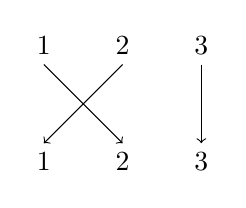
\begin{tikzpicture}
        \draw[->] (-1,1) node[above] {1} -- (0,0) node[below] {2};
        \draw[->] (0,1) node[above] {2} -- (-1,0) node[below] {1};
        \draw[->] (1,1) node[above] {3} -- (1,0) node[below] {3};
      \end{tikzpicture}

    \end{center}

  \end{enumerate}

\end{example}

The arrow diagram used to define the function above can be very helpful in visualizing functions.  We will often be working with functions on finite sets so this kind of picture is often more useful than a traditional graph of a function.  A graph of the function in example 3 above would look like this:

\begin{center}
  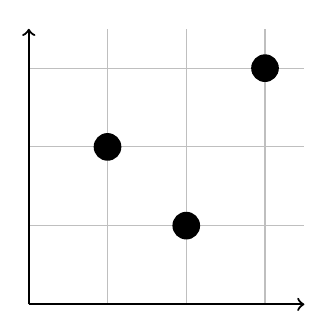
\begin{tikzpicture}
    %axis:
    \draw[thin, gray!50] (0,0) grid (3.5, 3.5);
    \draw[->, thick] (0,0) -- (0,3.5);
   \draw[->, thick] (0,0) -- (3.5,0);
   %points:
   \fill (1,2) circle (5pt) (2,1) circle (5pt) (3,3) circle (5pt);
  \end{tikzpicture}

\end{center}

It would be absolutely WRONG to connect the dots or try to fit them to some curve.  There are only three elements in the domain.  A curve suggests that the domain contains an entire interval of real numbers.  Remember, we are not in calculus any more!

It is important to know how to recognize a function from a rule which is not a function.  The arrow diagram can help.

\begin{example}
Which of the following diagrams represent a function.  Let $X = \{1,2,3,4\}$ and $Y = \{a,b,c,d\}$
  \begin{multicols}{3}
    \begin{center}
      $f:X \to Y$
      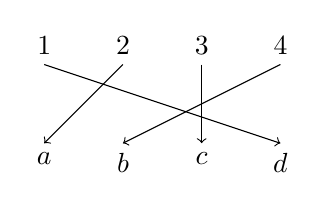
\begin{tikzpicture}
        \draw[->] (-1.5,1) node[above] {1} -- (1.5,0) node[below] {$d$};
        \draw[->] (-.5,1) node[above] {2} -- (-1.5,0) node[below] {$a$};
        \draw[->] (.5,1) node[above] {3} -- (.5, 0) node[below] {$c$};
        \draw[->] (1.5,1) node[above] {4} -- (-.5, 0) node[below] {$b$};
      \end{tikzpicture}
      \columnbreak
      
      $g:X \to Y$
	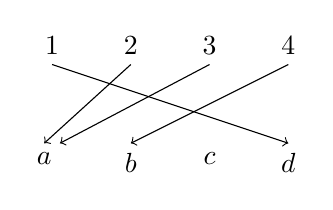
\begin{tikzpicture}
        \draw[->] (-1.5,1) node[above] {1} -- (1.5,0) node[below] {$d$};
        \draw[->] (-.5,1) node[above] {2} -- (-1.6,0) node[below] {$a$};
        \draw[->] (.5,1) node[above] {3} -- (-1.4, 0);
        \draw[->] (1.5,1) node[above] {4} -- (-.5, 0) node[below] {$b$};
        \draw (.5,0) node[below] {$c$};
      \end{tikzpicture}
      
      \columnbreak
      
      $h:X \to Y$
      	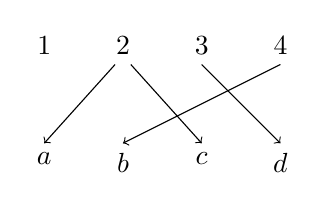
\begin{tikzpicture}
        \draw (-1.5,1) node[above] {1};
        \draw[->] (-.5,1) node[above] {2} (-.6,1) -- (-1.5,0) node[below] {$a$};
        \draw[->] (-.4,1) -- (.5,0);
        \draw[->] (.5,1) node[above] {3} -- (1.5, 0) node[below] {$d$};
        \draw[->] (1.5,1) node[above] {4} -- (-.5, 0) node[below] {$b$};
        \draw (.5,0) node[below] {$c$};
      \end{tikzpicture}
    \end{center}

  \end{multicols}
\begin{solution}
  $f$ is a function.  So is $g$.  There is no problem with an element of the codomain not being the output for any input, and there is no problem with $a$ from the codomain being the output of both 2 and 3 from the domain.  
  
  However, $h$ is \textbf{not} a function.  In fact, it fails for two reasons.  First, the element 1 from the domain has not been mapped to any element from the codomain.  Second, the element 2 from the domain has been mapped to more than one element from the codomain ($a$ and $c$).  Note that either one of these problems is enough to make a rule not a function.  Neither of these mappings are functions:
  \begin{center}
    \begin{multicols}{2}
      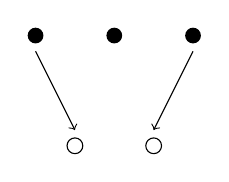
\begin{tikzpicture}
        \fill (-1, 1.2) circle (.1) (0,1.2) circle (.1) (1, 1.2) circle (.1);
        \draw[->] (-1, 1) -- (-.5,0);
        \draw[->] (1,1) -- (.5, 0);
        \draw (-.5, -0.2) circle (.1) (.5, -0.2) circle (.1);
      \end{tikzpicture}
       
       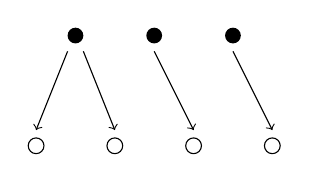
\begin{tikzpicture}
         \fill (-1, 1.2) circle (.1) (0,1.2) circle (.1) (1, 1.2) circle (.1);
         \draw[->] (-1.1, 1) -- (-1.5, 0);
         \draw[->] (-.9, 1) -- (-.5, 0);
         \draw[->] (0,1) -- (.5,0);
         \draw[->] (1,1) -- (1.5, 0);
         \draw (-.5, -0.2) circle (.1) (.5, -0.2) circle (.1) (-1.5, -0.2) circle (.1) (1.5, -0.2) circle (.1);
       \end{tikzpicture}

    \end{multicols}
  Not functions.
  \end{center}

\end{solution}

\end{example}

\subsection{Surjections, Injections, and Bijections}

We now turn to investigating special properties functions might or might not possess.  

In the examples above, you may have noticed that sometimes there are elements of the codomain which are not in the range.  When this sort of the thing \emph{does not} happen, (that is, when everything in the codomain is in the range) we say the function is \emph{onto}\index{onto|see {surjection}} or that the function maps the domain \emph{onto} the codomain.  This terminology should make sense: the function puts the domain (entirely) on top the codomain.  The fancy math term for an onto function is a \emph{surjection}\index{surjection}, and we say that an onto function is a \emph{surjective} function.

In pictures:

\begin{multicols}{2}
  \begin{center}
          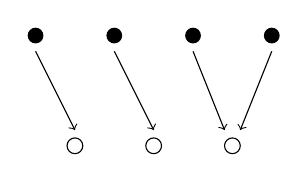
\begin{tikzpicture}
        \fill (-1.5, 1.2) circle (.1) (-.5,1.2) circle (.1) (.5, 1.2) circle (.1) (1.5,1.2) circle (.1);
        \draw[->] (-1.5, 1) -- (-1,0);
        \draw[->] (-.5,1) -- (0, 0);
        \draw[->] (.5, 1) -- (.9,0);
        \draw[->] (1.5,1) -- (1.1,0);
        \draw (-1, -0.2) circle (.1) (0, -0.2) circle (.1) (1, -0.2) circle (.1);
      \end{tikzpicture}
      
      Surjective
      
      \columnbreak
      
                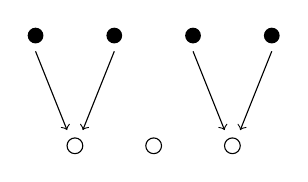
\begin{tikzpicture}
        \fill (-1.5, 1.2) circle (.1) (-.5,1.2) circle (.1) (.5, 1.2) circle (.1) (1.5,1.2) circle (.1);
        \draw[->] (-1.5, 1) -- (-1.1,0);
        \draw[->] (-.5,1) -- (-.9, 0);
        \draw[->] (.5, 1) -- (.9,0);
        \draw[->] (1.5,1) -- (1.1,0);
        \draw (-1, -0.2) circle (.1) (0, -0.2) circle (.1) (1, -0.2) circle (.1);
      \end{tikzpicture}
      
      Not surjective
  \end{center}

\end{multicols}

\begin{example}
  Which functions are surjective (i.e., onto)?
    \begin{enumerate}
    \item $f:\Z \to \Z$ defined by $f(n) = 3n$.  
    \item $g: \{1,2,3\} \to \{a,b,c\}$ defined by $g(1) = c$, $g(2) = a$ and $g(3) = a$.  
    \item $h:\{1,2,3\} \to \{1,2,3\}$ defined as follows:
    \begin{center}
      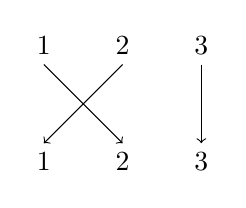
\begin{tikzpicture}
        \draw[->] (-1,1) node[above] {1} -- (0,0) node[below] {2};
        \draw[->] (0,1) node[above] {2} -- (-1,0) node[below] {1};
        \draw[->] (1,1) node[above] {3} -- (1,0) node[below] {3};
      \end{tikzpicture}
    \end{center}
  \end{enumerate}
  \begin{solution}
    \begin{enumerate}
      \item $f$ is not surjective.  There are elements in the codomain which are not in the range.  For example, no $n \in \Z$ gets mapped to the number 1 (the rule would say that $\frac{1}{3}$ would be sent to 1, but $\frac{1}{3}$ is not in the domain).  In fact, the range of the function is $3\Z$ (the integer multiples of 3), which is not equal to $\Z$.
      \item $g$ is not surjective.  There is no $x \in \{1,2,3\}$ (the domain) for which $g(x) = b$.  So $b$, which is in the codomain, is not in the range, so once again the function is not onto.
      \item $h$ is surjective.  Every element of the codomain is also in the range.  Nothing is missed.
    \end{enumerate}

  \end{solution}

\end{example}


To be a function, a map cannot assign a single element of the domain to two or more different elements of the codomain.  However, we have seen that the reverse is permissible.  That is, a function might assign the same element of the codomain to two or more different elements of the domain.  When this \emph{does not} occur (that is, when each element of the codomain is assigned to at most one element of the domain) then we say the function is \emph{one-to-one}\index{one-to-one|see {injection}}.  Again, this terminology makes sense: we are sending at most one element from the domain to one element from the codomain.  One input to one output. The fancy math term for a one-to-one function is an \emph{injection}\index{injection}.  We call one-to-one functions \emph{injective} functions.

In pictures:

\begin{multicols}{2}
  \begin{center}
          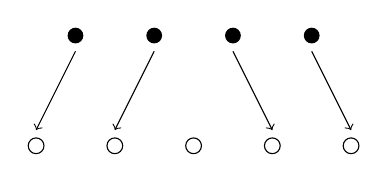
\begin{tikzpicture}
        \fill (-1.5, 1.2) circle (.1) (-.5,1.2) circle (.1) (.5, 1.2) circle (.1) (1.5,1.2) circle (.1);
        \draw[->] (-1.5, 1) -- (-2,0);
        \draw[->] (-.5,1) -- (-1, 0);
        \draw[->] (.5, 1) -- (1,0);
        \draw[->] (1.5,1) -- (2,0);
        \draw (-2, -0.2) circle (.1) (-1, -.2) circle (.1) (0, -0.2) circle (.1) (1, -0.2) circle (.1) (2, -0.2) circle (.1);
      \end{tikzpicture}
      
      Injective
      
      \columnbreak
      
                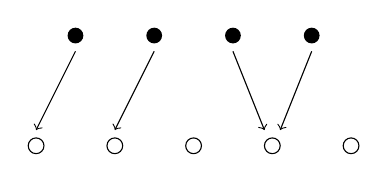
\begin{tikzpicture}
        \fill (-1.5, 1.2) circle (.1) (-.5,1.2) circle (.1) (.5, 1.2) circle (.1) (1.5,1.2) circle (.1);
        \draw[->] (-1.5, 1) -- (-2,0);
        \draw[->] (-.5,1) -- (-1, 0);
        \draw[->] (.5, 1) -- (.9,0);
        \draw[->] (1.5,1) -- (1.1,0);
        \draw (-2, -0.2) circle (.1) (-1, -.2) circle (.1) (0, -0.2) circle (.1) (1, -0.2) circle (.1) (2, -0.2) circle (.1);
      \end{tikzpicture}
      
      Not injective
  \end{center}

\end{multicols}


\begin{example}
  Which functions are injective (i.e., one-to-one)?
    \begin{enumerate}
    \item $f:\Z \to \Z$ defined by $f(n) = 3n$.  
    \item $g: \{1,2,3\} \to \{a,b,c\}$ defined by $g(1) = c$, $g(2) = a$ and $g(3) = a$.  
    \item $h:\{1,2,3\} \to \{1,2,3\}$ defined as follows:
    \begin{center}
      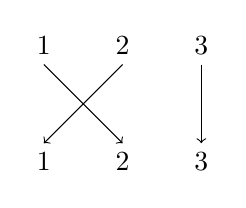
\begin{tikzpicture}
        \draw[->] (-1,1) node[above] {1} -- (0,0) node[below] {2};
        \draw[->] (0,1) node[above] {2} -- (-1,0) node[below] {1};
        \draw[->] (1,1) node[above] {3} -- (1,0) node[below] {3};
      \end{tikzpicture}
    \end{center}
  \end{enumerate}
  \begin{solution}
    \begin{enumerate}
      \item $f$ is injective.  Each element in the codomain is assigned to at \emph{most} one element from the domain.  If $x$ is a multiple of three, then only $x/3$ is mapped to $x$.  If $x$ is not a multiple of 3, then there is no input corresponding to the output $x$.
      \item $g$ is not injective.  Both inputs $2$ and $3$ are assigned the output $a$.
      \item $h$ is injective.  Each output is only an output once.
    \end{enumerate}

  \end{solution}

\end{example}



From the examples above, it should be clear that there are functions which are surjective, injective, both or neither.  In the case when a function is both one-to-one and onto (a injection and surjection) we say the function is a \emph{bijection}, or that the function is a \emph{bijective} function.  

\subsection{Inverse Image}

When discussing functions, we have notation for talking about an element of the domain (say $x$) and its corresponding element in the codomain (we write $f(x)$).  It would also be nice to start with some element of the codomain (say $y$) and talk about which element or elements (if any) from the domain get sent to it.  We could write ``those $x$ in the domain such that $f(x) = y$,'' but this is a lot of writing.  So here is some notation to make our lives easier.

Suppose $f:X \to Y$ is a function.  For $y \in Y$ (an element of the codomain), we write $f\inv(y)$ to represent the \emph{set} of all elements in the domain $X$ which get sent to $y$.  That is, $f\inv(y) = \{x \in X \st f(x) = y\}$.  We say that $f\inv(y)$ is the \emph{complete inverse image}\index{inverse image} of $y$ under $f$.

\vskip 1em
\noindent\textbf{WARNING: $f\inv(y)$ is not an inverse function!!!!  Inverse functions only exist for bijections, but $f\inv(y)$ is defined for any function $f$.  The point: $f\inv(y)$ is a \underline{set}, not an element of the domain.}
\vskip 1em

\begin{example}
 Consider the function $f:\{1,2,3,4,5,6\} \to \{a,b,c,d\}$ given by $f(1) = a$, $f(2) = a$, $f(3) = b$, $f(4) = c$, $f(5) = c$ and $f(6) = c$.  Find the complete inverse image of each element in the codomain.
 \begin{solution}
  Remember, we are looking for sets.
  \[f\inv(a) = \{1,2\}\]
  \[f\inv(b) = \{3\}\]
  \[f\inv(c) = \{4,5,6\}\]
  \[f\inv(d) = \emptyset.\]
 \end{solution}
\end{example}

\begin{example} Consider the function $g:\Z \to \Z$ defined by $g(n) = n^2 + 1$.  Find $g\inv(1)$, $g\inv(2)$, $g\inv(3)$ and $g\inv(10)$.
 \begin{solution}
  To find $g\inv(1)$, we need to find all integers $n$ such that $n^2 + 1 = 1$.  Clearly only 0 works, so $g\inv(1) = \{0\}$ (note that even though there is only one element, we still write it as a set with one element in it).  
  
  To find $g\inv(2)$, we need to find all $n$ such that $n^2 + 1 = 2$.  We see $g\inv(2) = \{-1,1\}$.  
  
  If $n^2 + 1 = 3$, then we are looking for an $n$ such that $n^2 = 2$.  There are no such integers so $g\inv(3) = \emptyset$. 
  
  Finally, $g\inv(10) = \{-3, 3\}$ because $g(-3) = 10$ and $g(3) = 10$.
 \end{solution}

\end{example}

Since $f\inv(y)$ is a set, it makes sense to ask for $|f\inv(y)|$, the number of elements in the domain which map to $y$.

\begin{example}
 Find a function $f:\{1,2,3,4,5\} \to \N$ such that $|f\inv(7)| = 5$.  
 \begin{solution}
 There is only one such function.  We need five elements of the domain to map to the number $7 \in \N$.  Since there are only five elements in the domain, all of them must map to 7.  So $f(1) = 7$, $f(2) = 7$, $f(3) = 7$, $f(4) = 7$ and $f(5) = 7$.
 \end{solution}
\end{example}





\begin{defbox}{Function Definitions}
\begin{itemize}
  \item A \emph{function} is a rule that assigns each element of a set, called the \emph{domain}, to exactly one element of a second set, called the \emph{codomain}.
  \item Notation: $f:X \to Y$ is our way of saying that the function is called $f$, the domain is the set $X$ and the codomain is the set $Y$.
  \item $f(x) = y$ means the element $x$ of the domain (input) is assigned to the element $y$ of the codomain.  We say $y$ is an output.  Alternatively, we call $y$ the \emph{image of $x$ under $f$}.
  \item The \emph{range} is a subset of the codomain.  It is the set of all elements which are assigned to at least one element of the domain by the function.  That is, the range is the set of all outputs.
  \item A function is \emph{injective} (an \emph{injection} or \emph{one-to-one}) if every element of the codomain is the output for \textbf{at most} one element from the domain.
  \item A function is \emph{surjective} (a \emph{surjection} or \emph{onto}) if every element of the codomain is the output of \textbf{at least} one element of the domain.
  \item A \emph{bijection} is a function which is both an injection and surjection.  In other words, if every element of the codomain is the output of \textbf{exactly one} element of the domain.
  \item The \emph{complete inverse image} of an element in the codomain, written $f\inv(y)$ is the \textbf{set} of all element in the domain which are assigned to $y$ by the function.  
\end{itemize}

\end{defbox}



\end{document}



%This, however, is far from the only reason you should study the subject.
%
%\section{Why Study Discrete Math?}
%
%There are two main reasons you should want to study discrete math.  First, discrete math is useful!  Lots of real world problems can be modeled using discrete math much more effectively than, say, calculus.
%




\end{document}
